\documentclass[12pt,a4paper]{scrartcl}

\usepackage[a4paper, left=2cm, right=2cm, bottom=1cm, top=1cm, includeheadfoot]{geometry}
\usepackage[ngerman]{babel}
\usepackage[utf8]{inputenc} % comment this if you uncomment utf8x
%\usepackage[utf8x]{inputenc} % uncomment this if there are problems with 'ä', 'ü', 'ö'
\usepackage{ucs}
\usepackage[usenames,dvipsnames]{xcolor}
\usepackage[fleqn]{amsmath}
\usepackage{amsfonts}
\usepackage{amssymb}
\usepackage{color}
\usepackage{listings}
\usepackage{hyperref}
\usepackage{amsfonts}
\usepackage{listings}
\usepackage{scrpage2}
\usepackage{graphicx}
\usepackage{pdfpages}
\usepackage{mathtools}
\usepackage{multirow}
\usepackage{float}
\usepackage{matlab-prettifier}


\definecolor{mygray}{rgb}{0.9,0.9,0.9}
\lstset{language=[Visual]Basic, morekeywords={param, local}}


\lstset{
   literate={ö}{{\"o}}1
           {ä}{{\"a}}1
           {ü}{{\"u}}1
           {ß}{{\ss}}1
           {é}{{\'e}}1,
   inputencoding=ansinew,
   extendedchars=true,
   basicstyle=\scriptsize\ttfamily,
   numberstyle=\scriptsize,
   breaklines=true,
   tabsize=4,
   numbersep=5pt
}
\lstdefinestyle{customcpp}{
   language=C++,
   backgroundcolor=\color{mygray},
   numbers=left,
   keywordstyle=\color{blue}\bfseries,
   stringstyle=\color{BrickRed}\ttfamily,
   commentstyle=\color{OliveGreen}\ttfamily,
   showspaces=false,
   showstringspaces=false,
   showtabs=false
}
\lstdefinestyle{customoutput}{
   backgroundcolor=\color{mygray},
   numbers=none,
   showspaces=false,
   showtabs=false
}

\newcommand{\sourceCode}[1]{\lstinputlisting[style=customcpp]{#1}}
\begin{document}

\title{SCD5 - Matlab - Übung 2}
\date{19. Oktober 2017}
\author{Daniel Klepatsch \and Thomas Reisinger}
        
\maketitle

\newpage

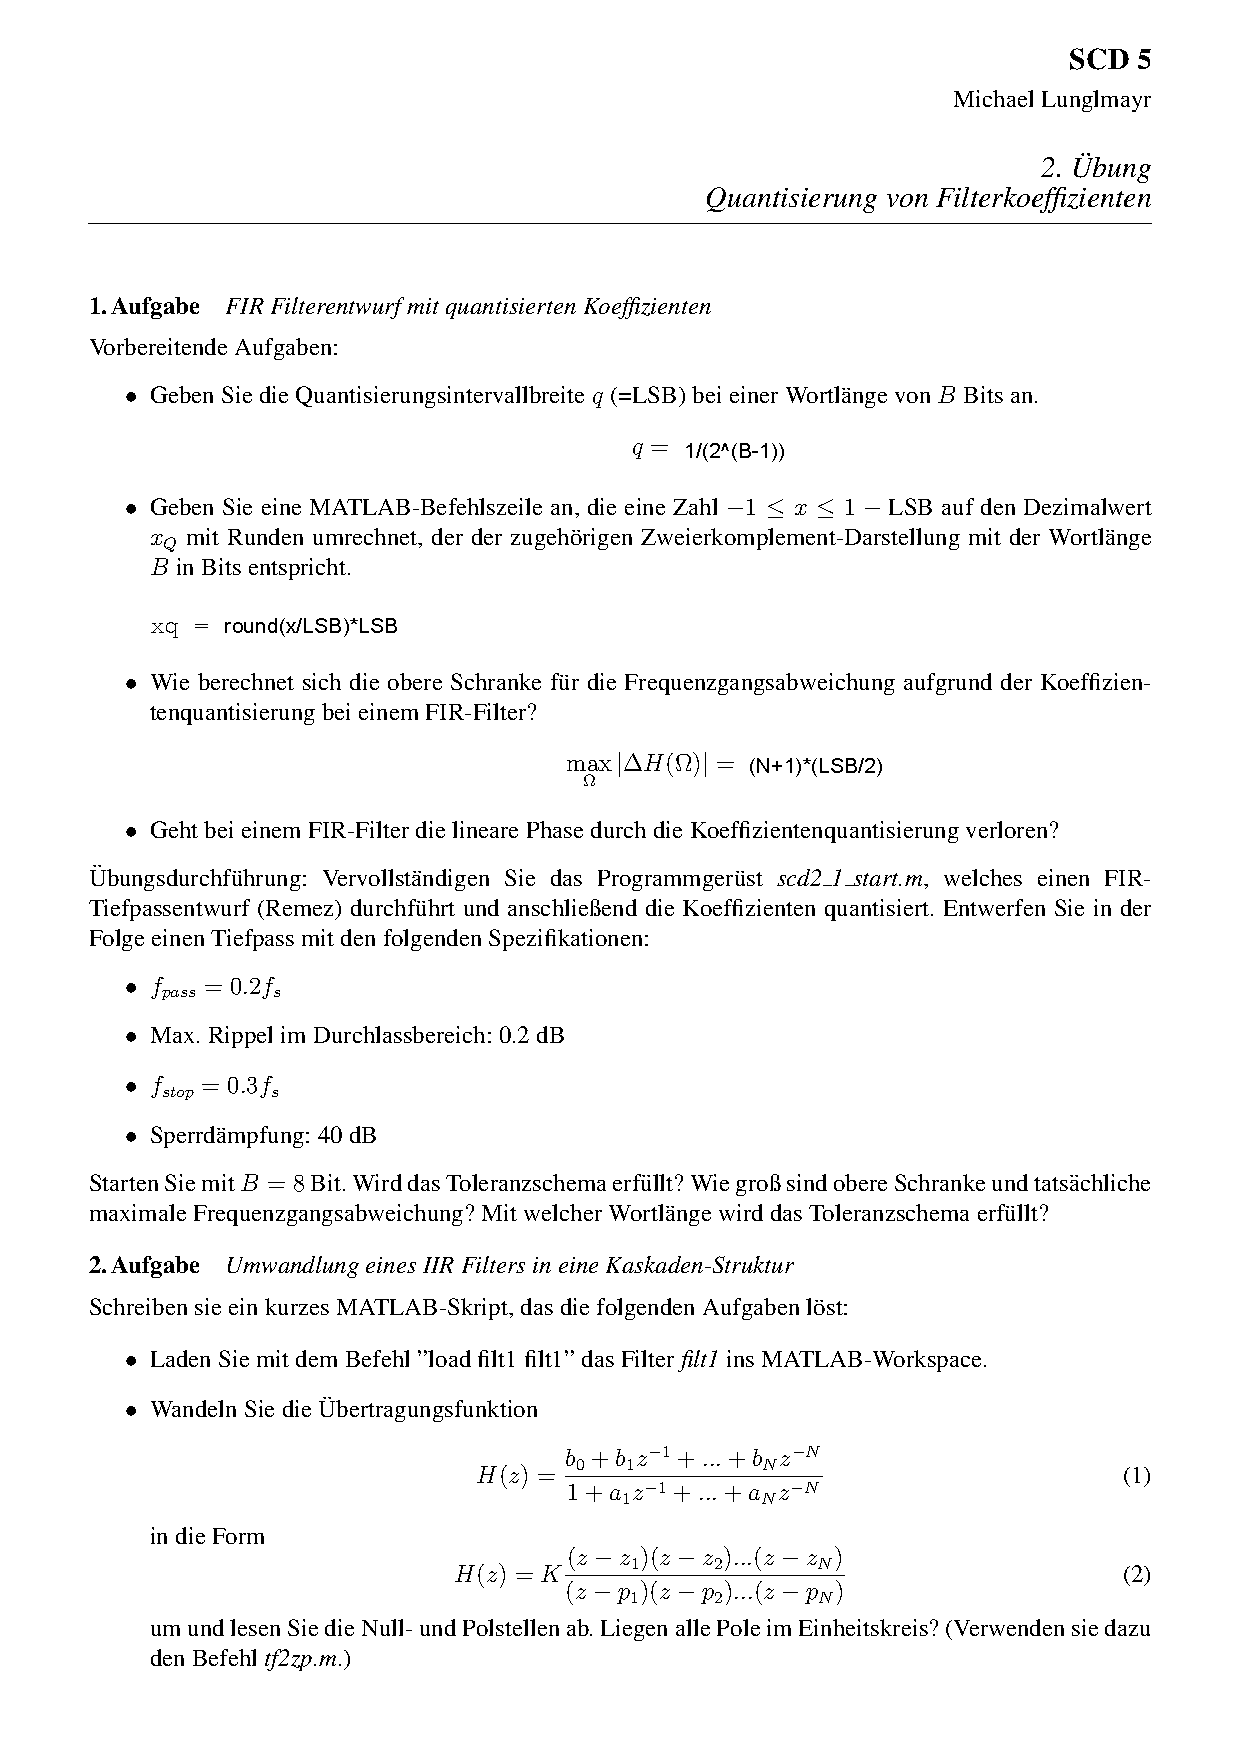
\includepdf[pages=-]{SCD_UE02_Deckblatt.pdf}

\tableofcontents

\newpage

\section{Aufgabe 1}

\begin{itemize}
\item Geht bei einem FIR-Filter die lineare Ohase durch die Koeffizientenquantisierung verloren?

Symmetrische FIR-filter weisen (abgesehen von 180-Grad-Phasensprüngen) einen linearen Phasengang auf. Durch die Quantisierung ändert sich allerdings nichts an der Symmetrie des Filter, nur an den einzelnen Faktoren. Das führ zu einem geänderten Verhalten des Filters. Die Linearphasigkeit geht aber nicht verloren.
\newline
\item Wird das Toleranzschema erfüllt?

Bei den Standardwerten aus der Angabe wird das Toleranzschema \textbf{nicht} eingehalten.
\newline
\item Wie groß sind die obere Schranke und tatsächliche maximale Frequenzgangabweichung?

Der Wert für die obere Schranke beträgt \textbf{4.00391}, ist aber der worst-case, der eintreten kann. Die tatsächliche Frequenzgangabweichung beträgt \textbf{0.030886}.
\newline
\item Mit welcher Wortlänge wird das Toleranzschema erfüllt?

Das Toleranzschema wird ab einer Wortlänge von 15 Bit erfüllt, dann treten keine Fehler mehr auf.
\end{itemize}

\subsection{Screenshots}

Das Skript mit Standardwerten und 8 Bit liefert folgendes Bild:
\begin{center}
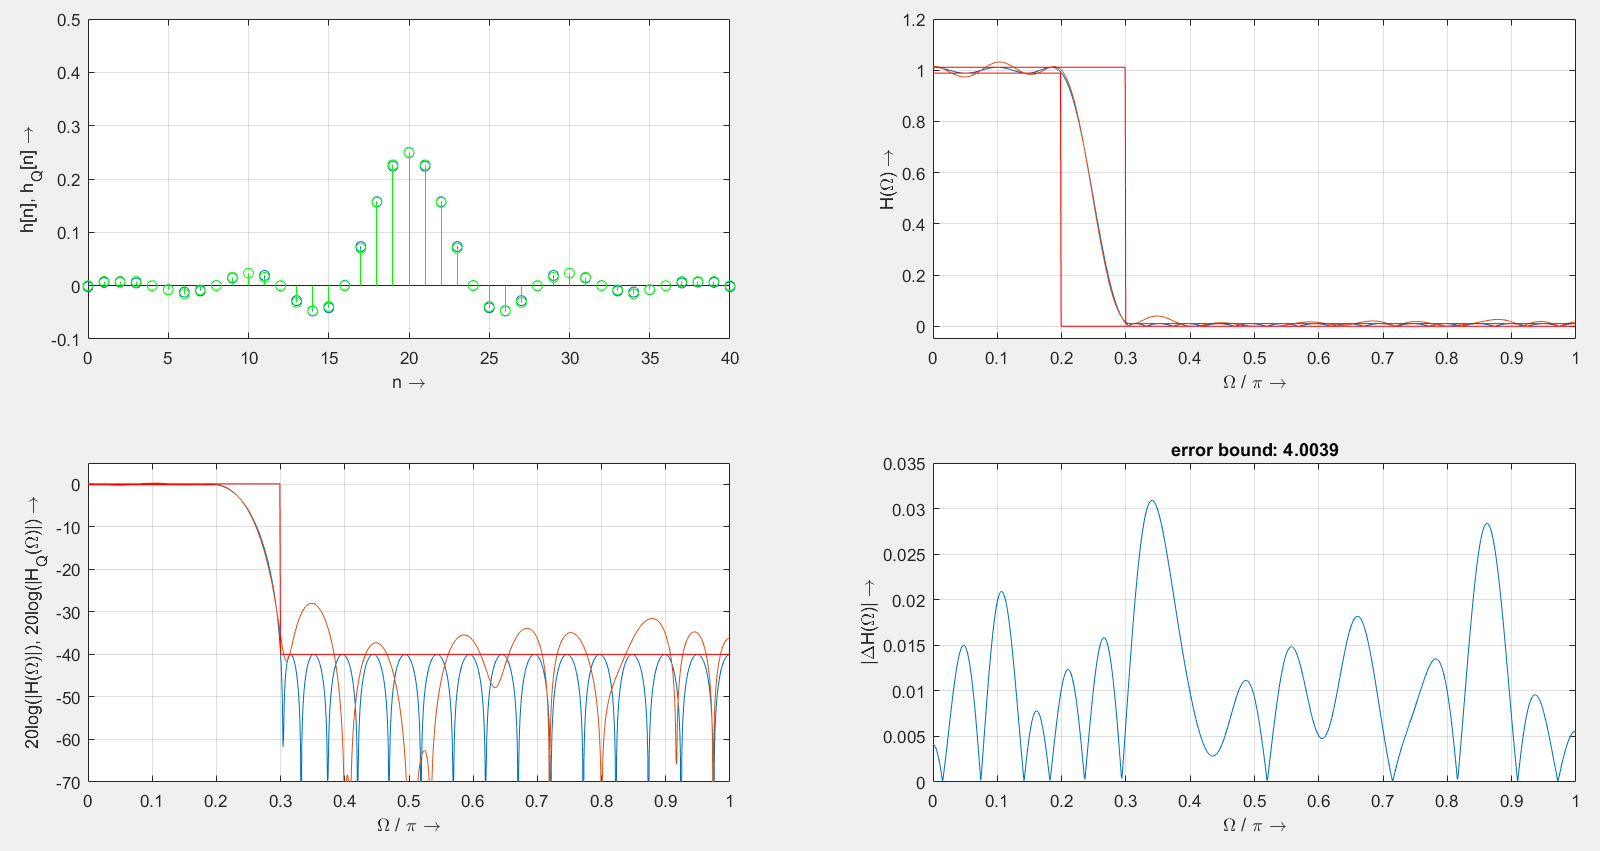
\includegraphics[scale=0.52]{UE02_1_8Bit.png}
\end{center}

\newpage

Das Skript mit Standardwerten und 15 Bit liefert folgendes Bild:
\begin{center}
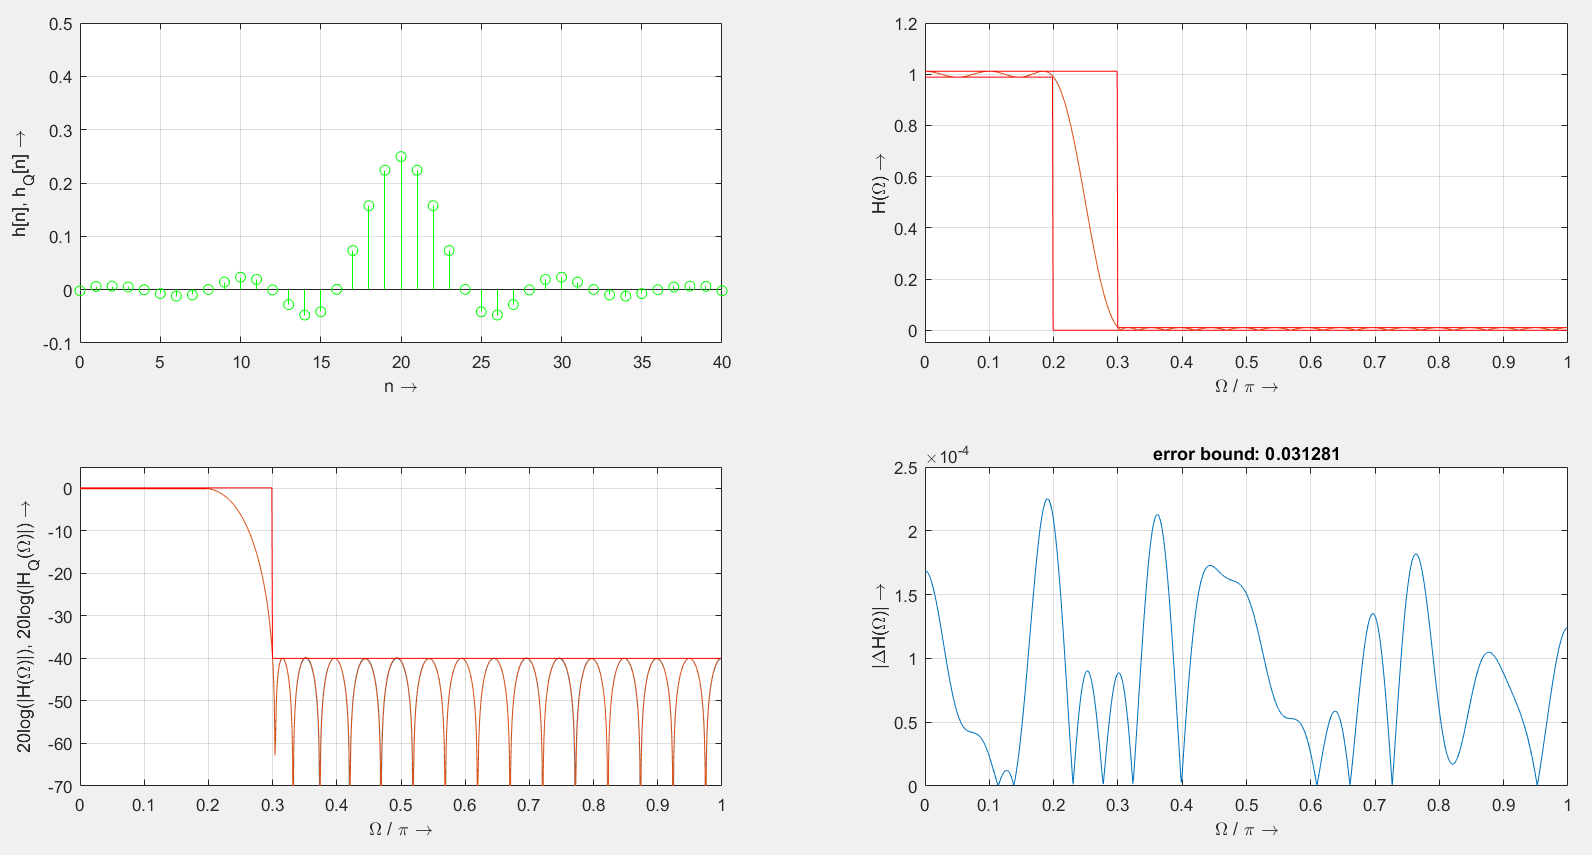
\includegraphics[scale=0.52]{UE02_1_15Bit.png}
\end{center}

\subsection{Konsolenausgaben}

Konsolenausgabe bei 8 Bit:
\sourceCode{UE02_1_8Bit.txt}

Konsolenausgabe bei 15 Bit:
\sourceCode{UE02_1_15Bit.txt}

\subsection{Matlab-Skript}

\sourceCode{../../workspace/scd2_1_start.m}

\newpage

\section{Aufgabe 2}

\subsection{Screenshots}

Pol-Nullstellten Diagramm des gesamten Filters:
\begin{center}
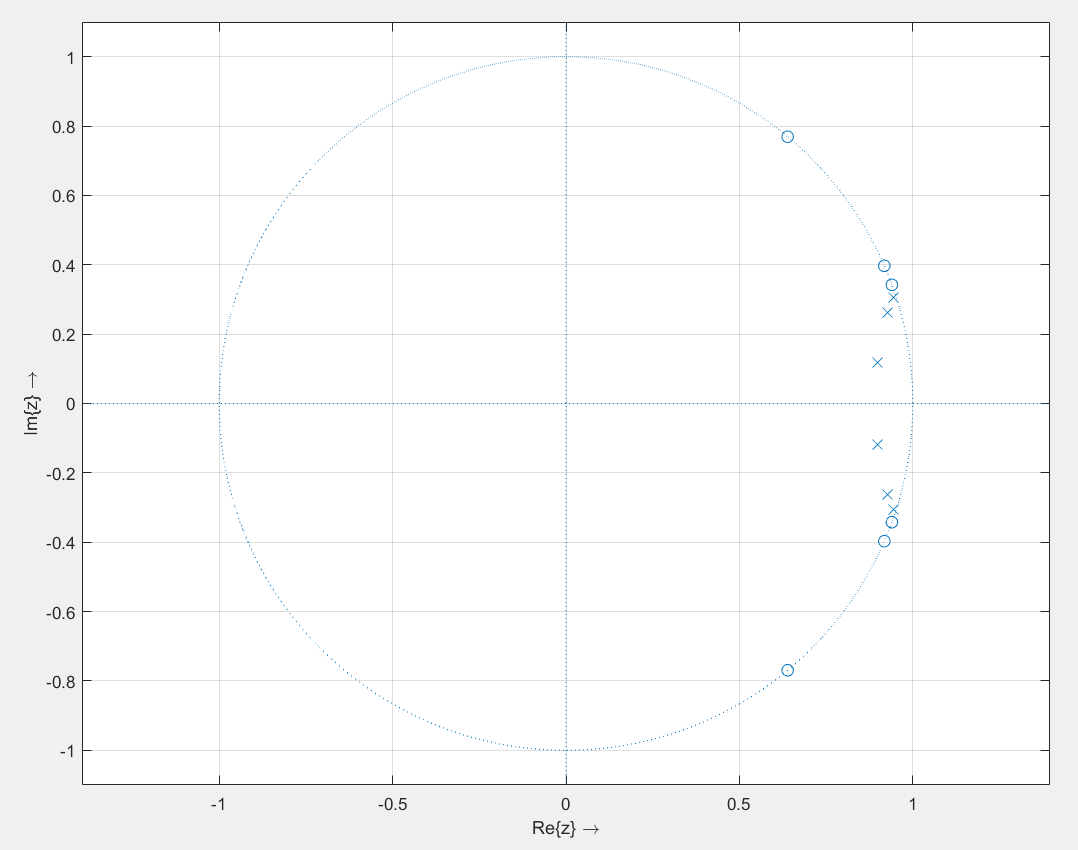
\includegraphics[scale=0.52]{UE02_2_filt1_zplane.png}
\end{center}

Pol-Nullstellten Diagramme der 2.-Ordnung-Subsysteme:
\begin{center}
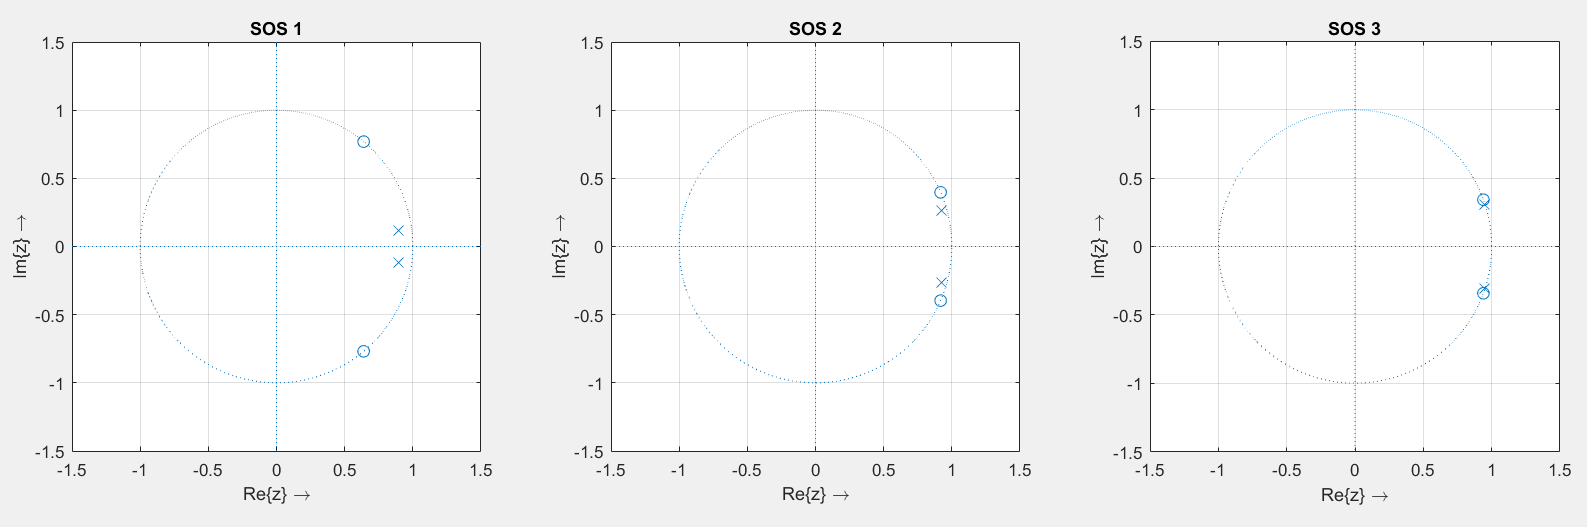
\includegraphics[scale=0.52]{UE02_2_SOS123_zplane.png}
\end{center}

\newpage

Amplitudengänge der 2.-Ordnung-Subsysteme:
\begin{center}
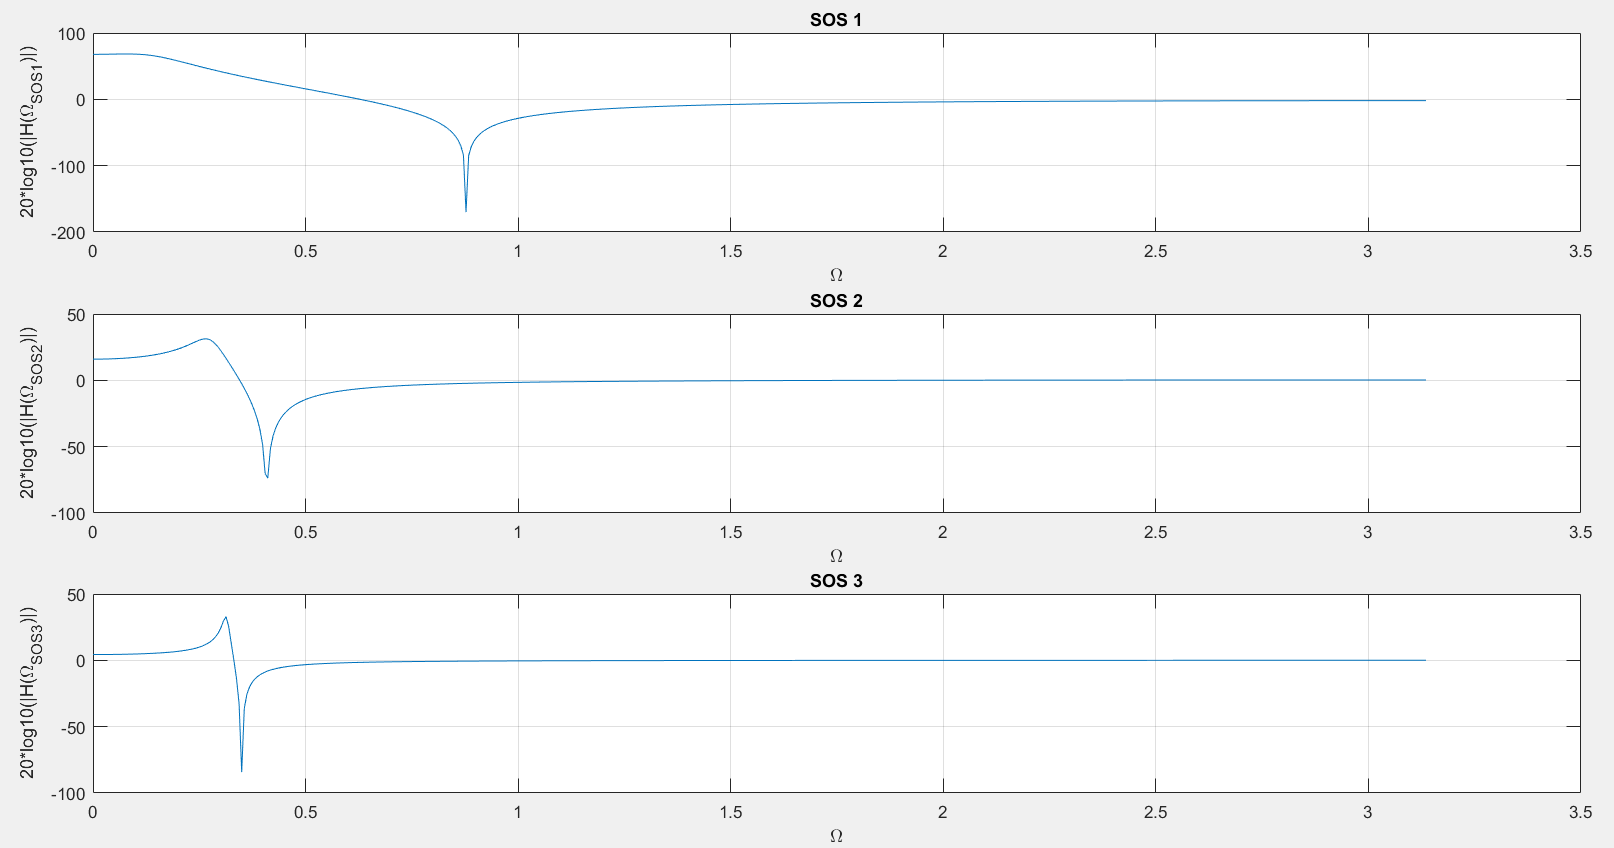
\includegraphics[scale=0.52]{UE02_2_SOS123_amp.png}
\end{center}

Amplitudengänge des Filters und der System aus 2.Ordnung-Subsystemen:
\begin{center}
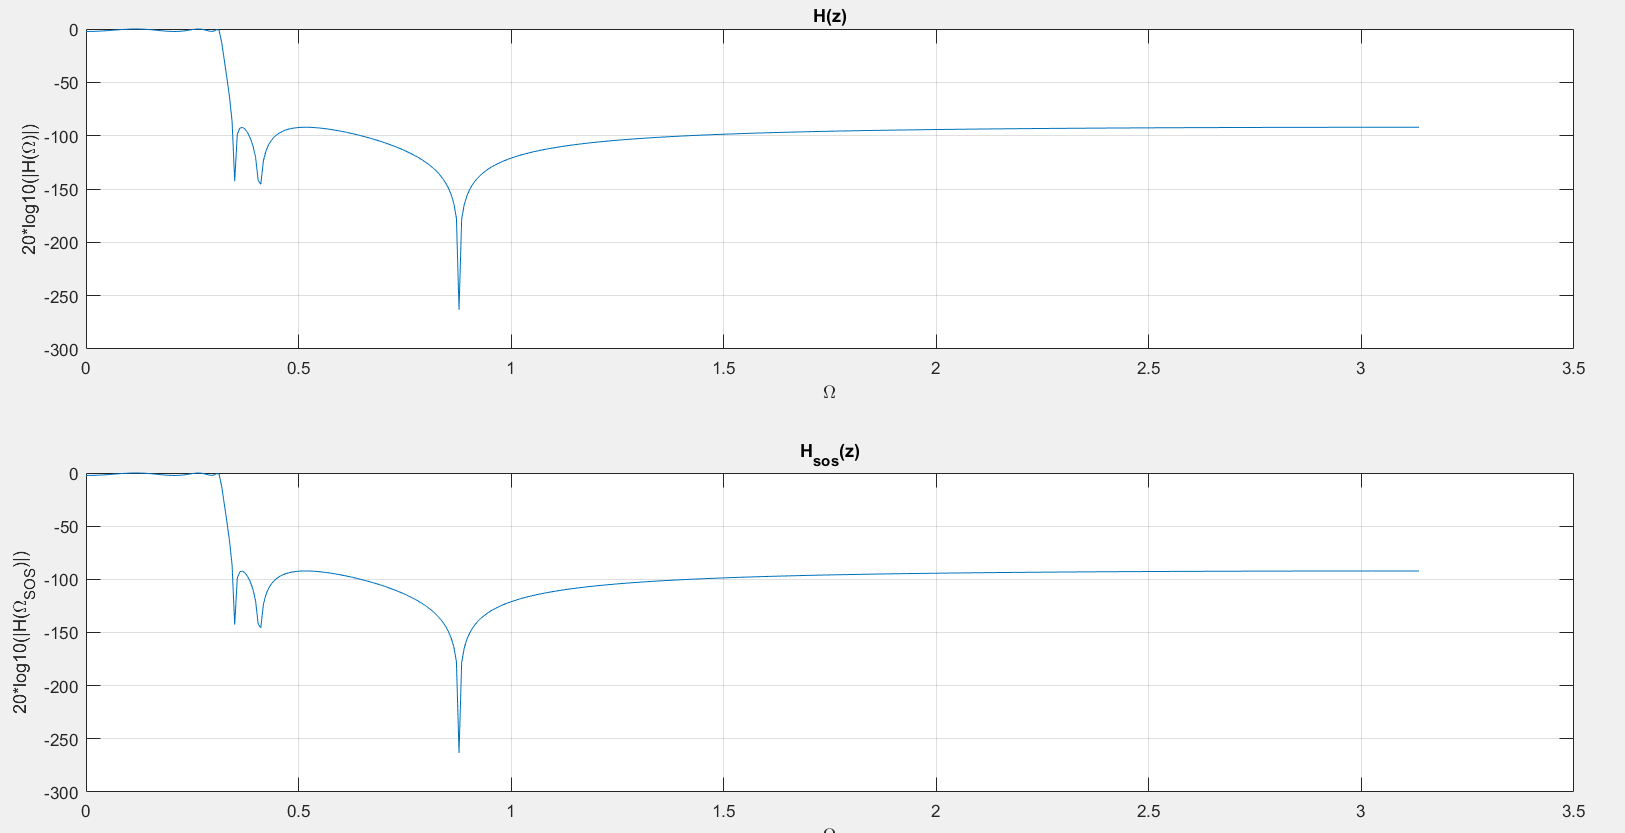
\includegraphics[scale=0.52]{UE02_2_H_H_sos_amp.png}
\end{center}

\newpage

\subsection{Konsolenausgaben}

\sourceCode{UE02_2_output.txt}

\newpage

\subsection{Matlab-Skript}

\sourceCode{../../workspace/scd2_2_start.m}

\subsection{Blockschalttbild Kaskaden-Struktur}

\begin{center}
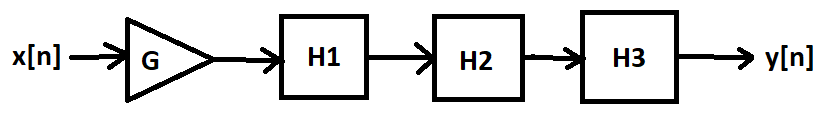
\includegraphics[scale=0.92]{UE02_2_Blockschaltbild.png}
\end{center}

\newpage

\section{Aufgabe 3}

\begin{itemize}
\item Wird das Toleranzschema mit beiden Implementierungen erfüllt?

Die direkte Implementierung erfüllt das Toleranzschema nicht.\\
Die kaskadierte Implementierung erfüllt das Toleranzschema.
\newline
\item Wie groß sind die maximalen Frequenzgangabweichung der beiden Implementierungen?

Direkte Implementierung: 0.131501\\
Kaskaden Implementierung: 0.00765129
\newline
\item Beobachtung bei Verringerung der Wortlänge

Bei Filtern mit vielen Koeffizienten oder kleinen Wortlängen hilft Kaskadierung den Quantisierungsfehler klein zu halten.
\end{itemize}

\newpage

\subsection{Screenshots}

Vergleich direkte Implementierung mit kasakadierter Implementierung:\\\\
Wortlänge 16 Bit:\\
\begin{center}
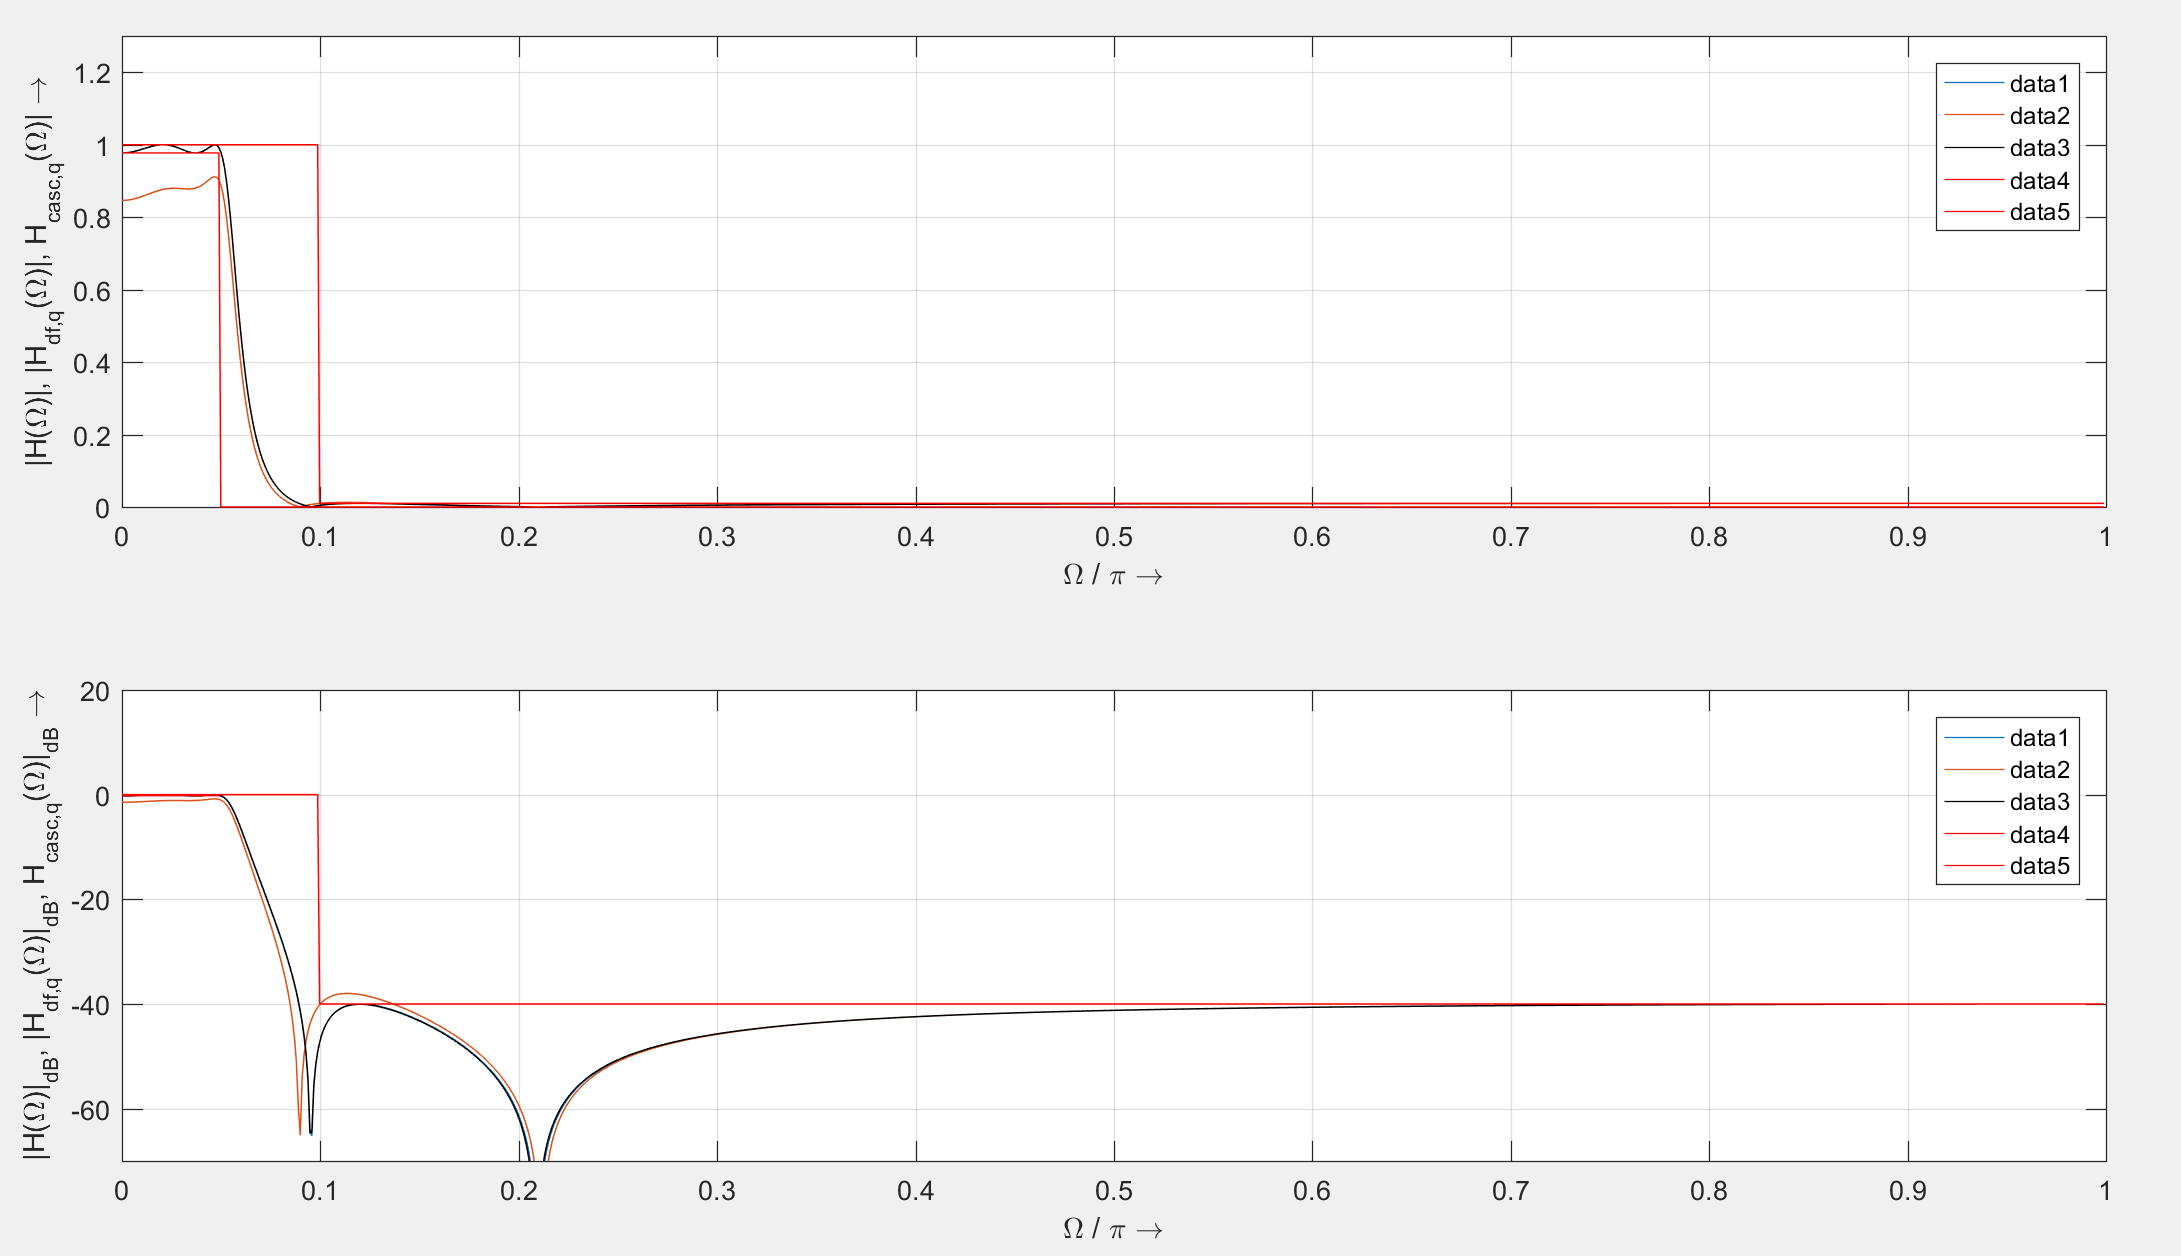
\includegraphics[scale=0.55]{UE02_3_16Bit.PNG}
\end{center}
Wortlänge 8 Bit:\\
\begin{center}
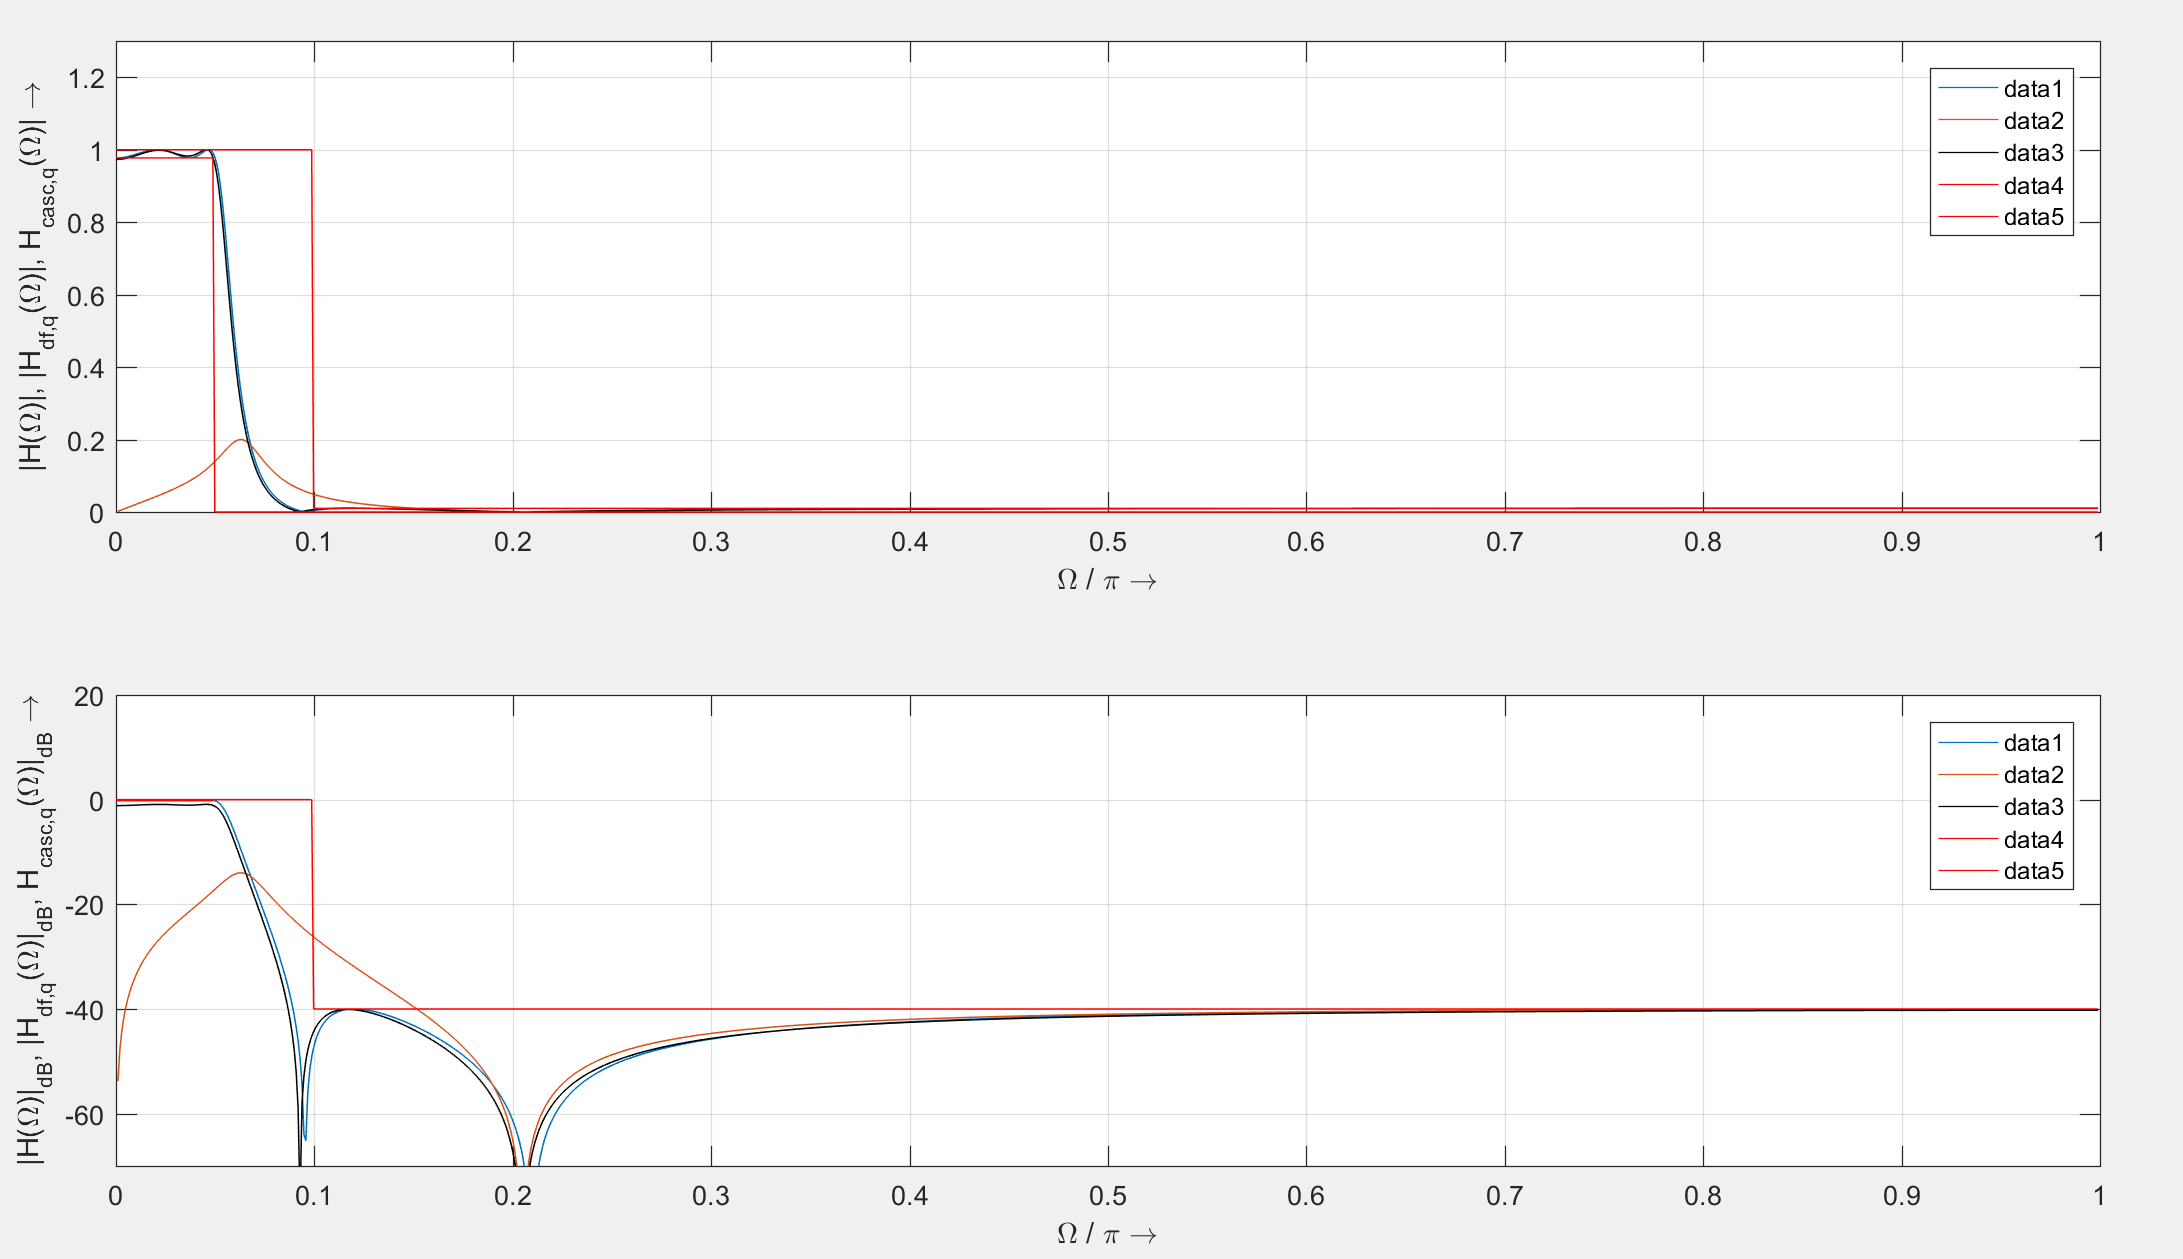
\includegraphics[scale=0.55]{UE02_3_10Bit.PNG}
\end{center}

\newpage

\begin{center}
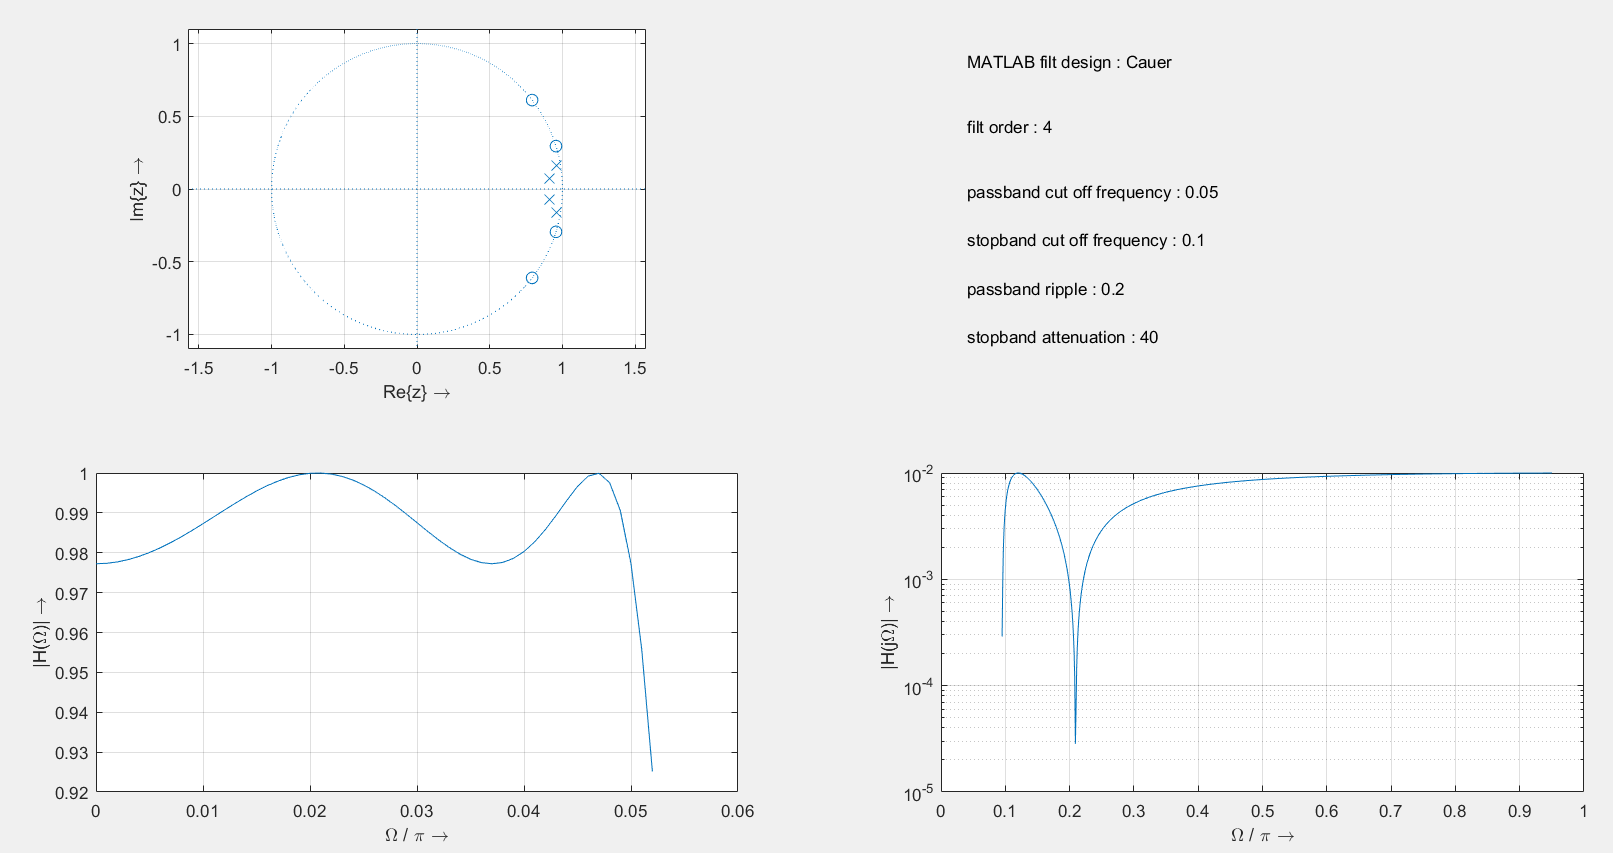
\includegraphics[scale=0.5]{UE02_3_Cauer.PNG}
\end{center}

\begin{center}
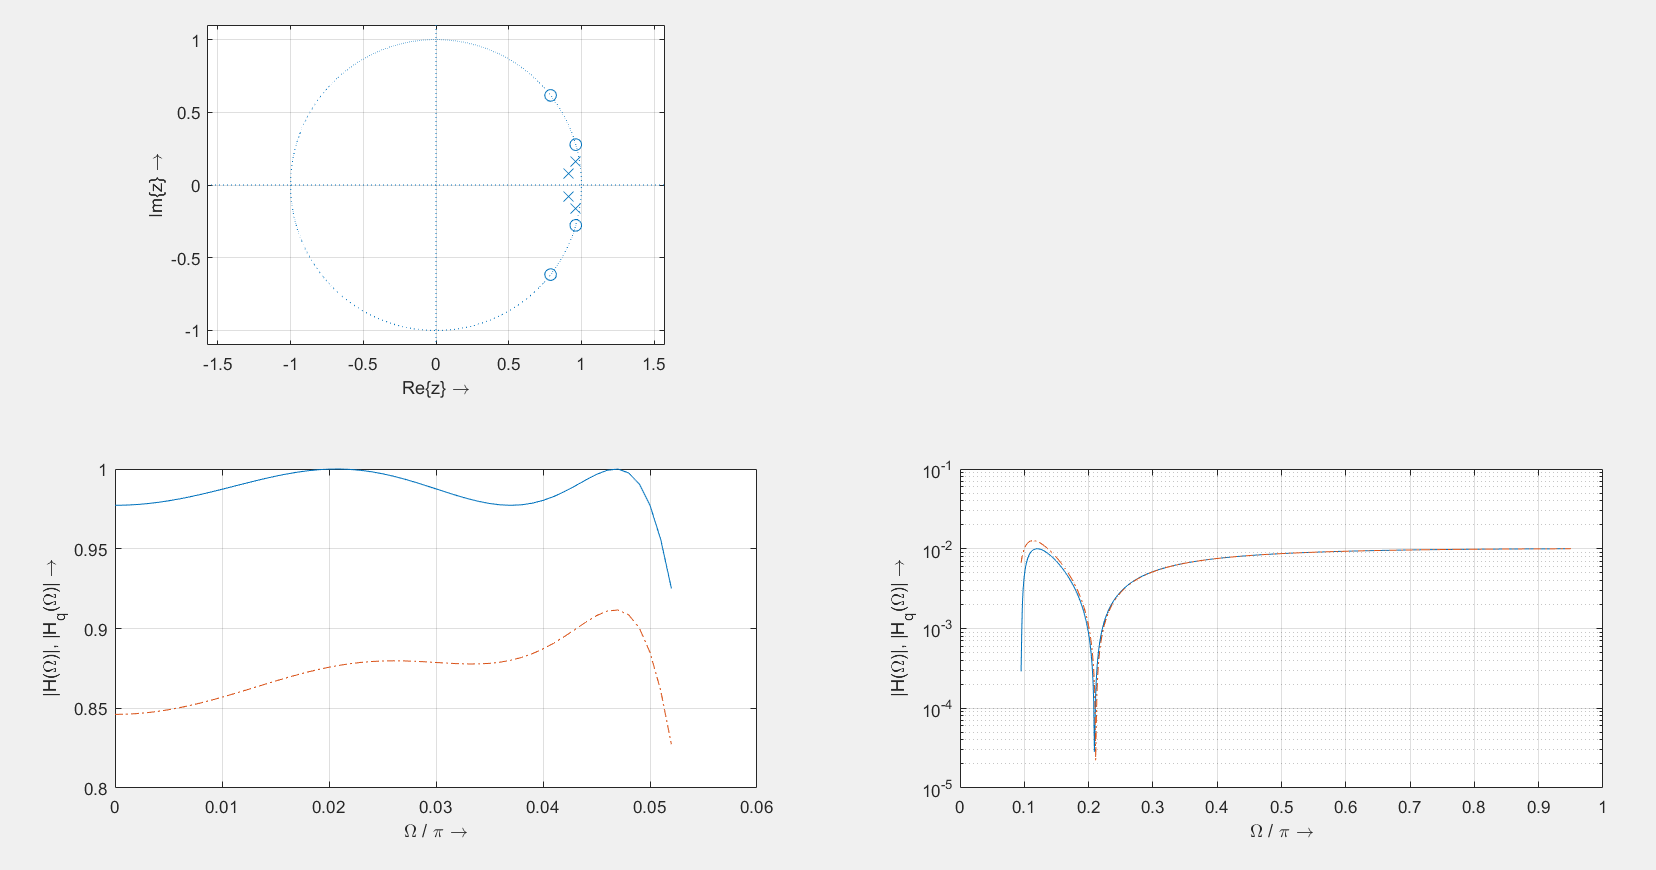
\includegraphics[scale=0.5]{UE02_3_Direct.PNG}
\end{center}

\begin{center}
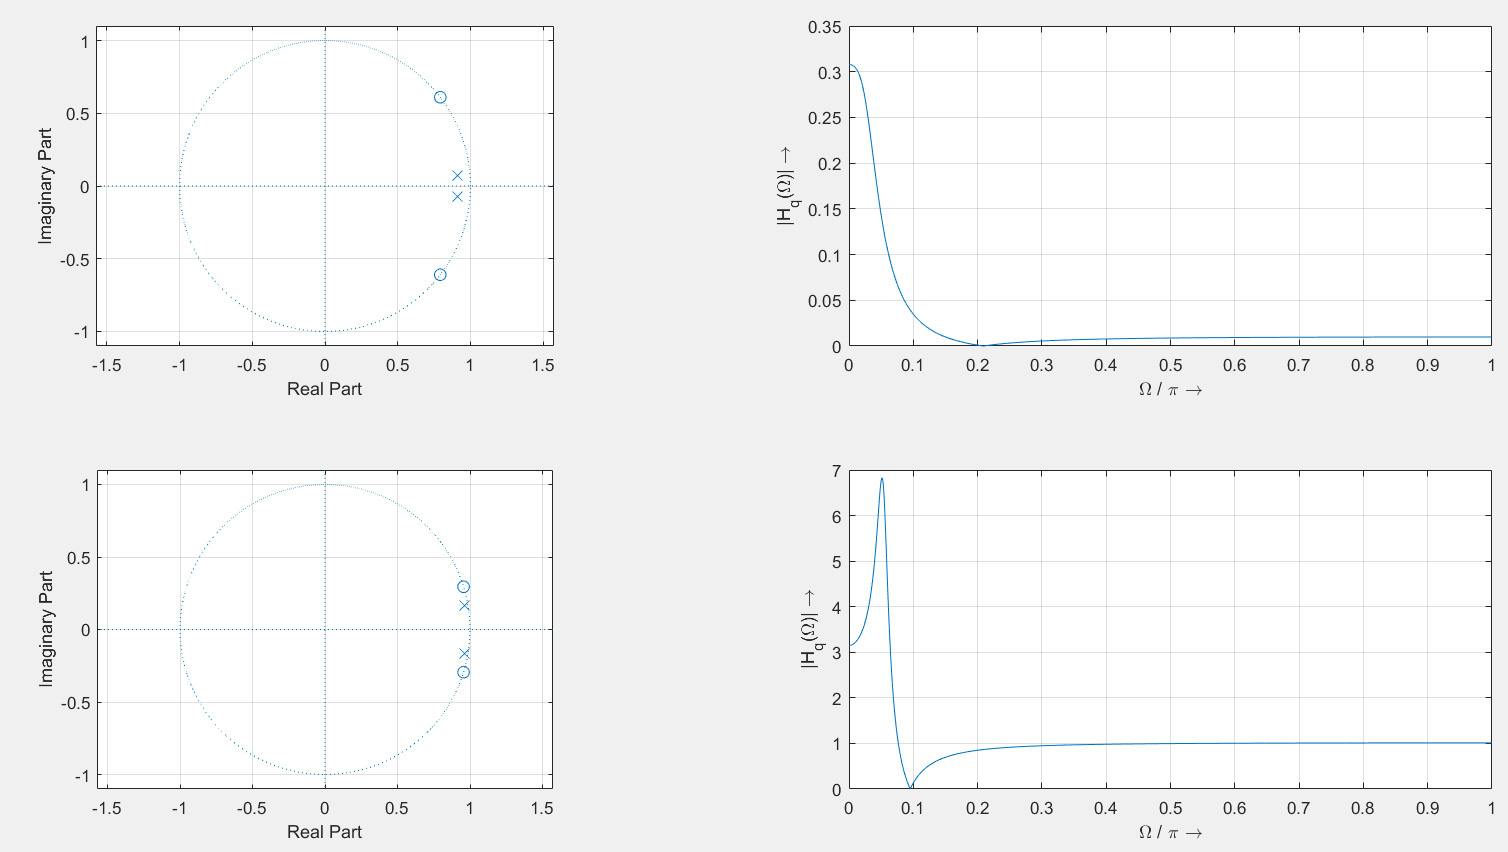
\includegraphics[scale=0.5]{UE02_3_Cascade_2.PNG}
\end{center}

\begin{center}
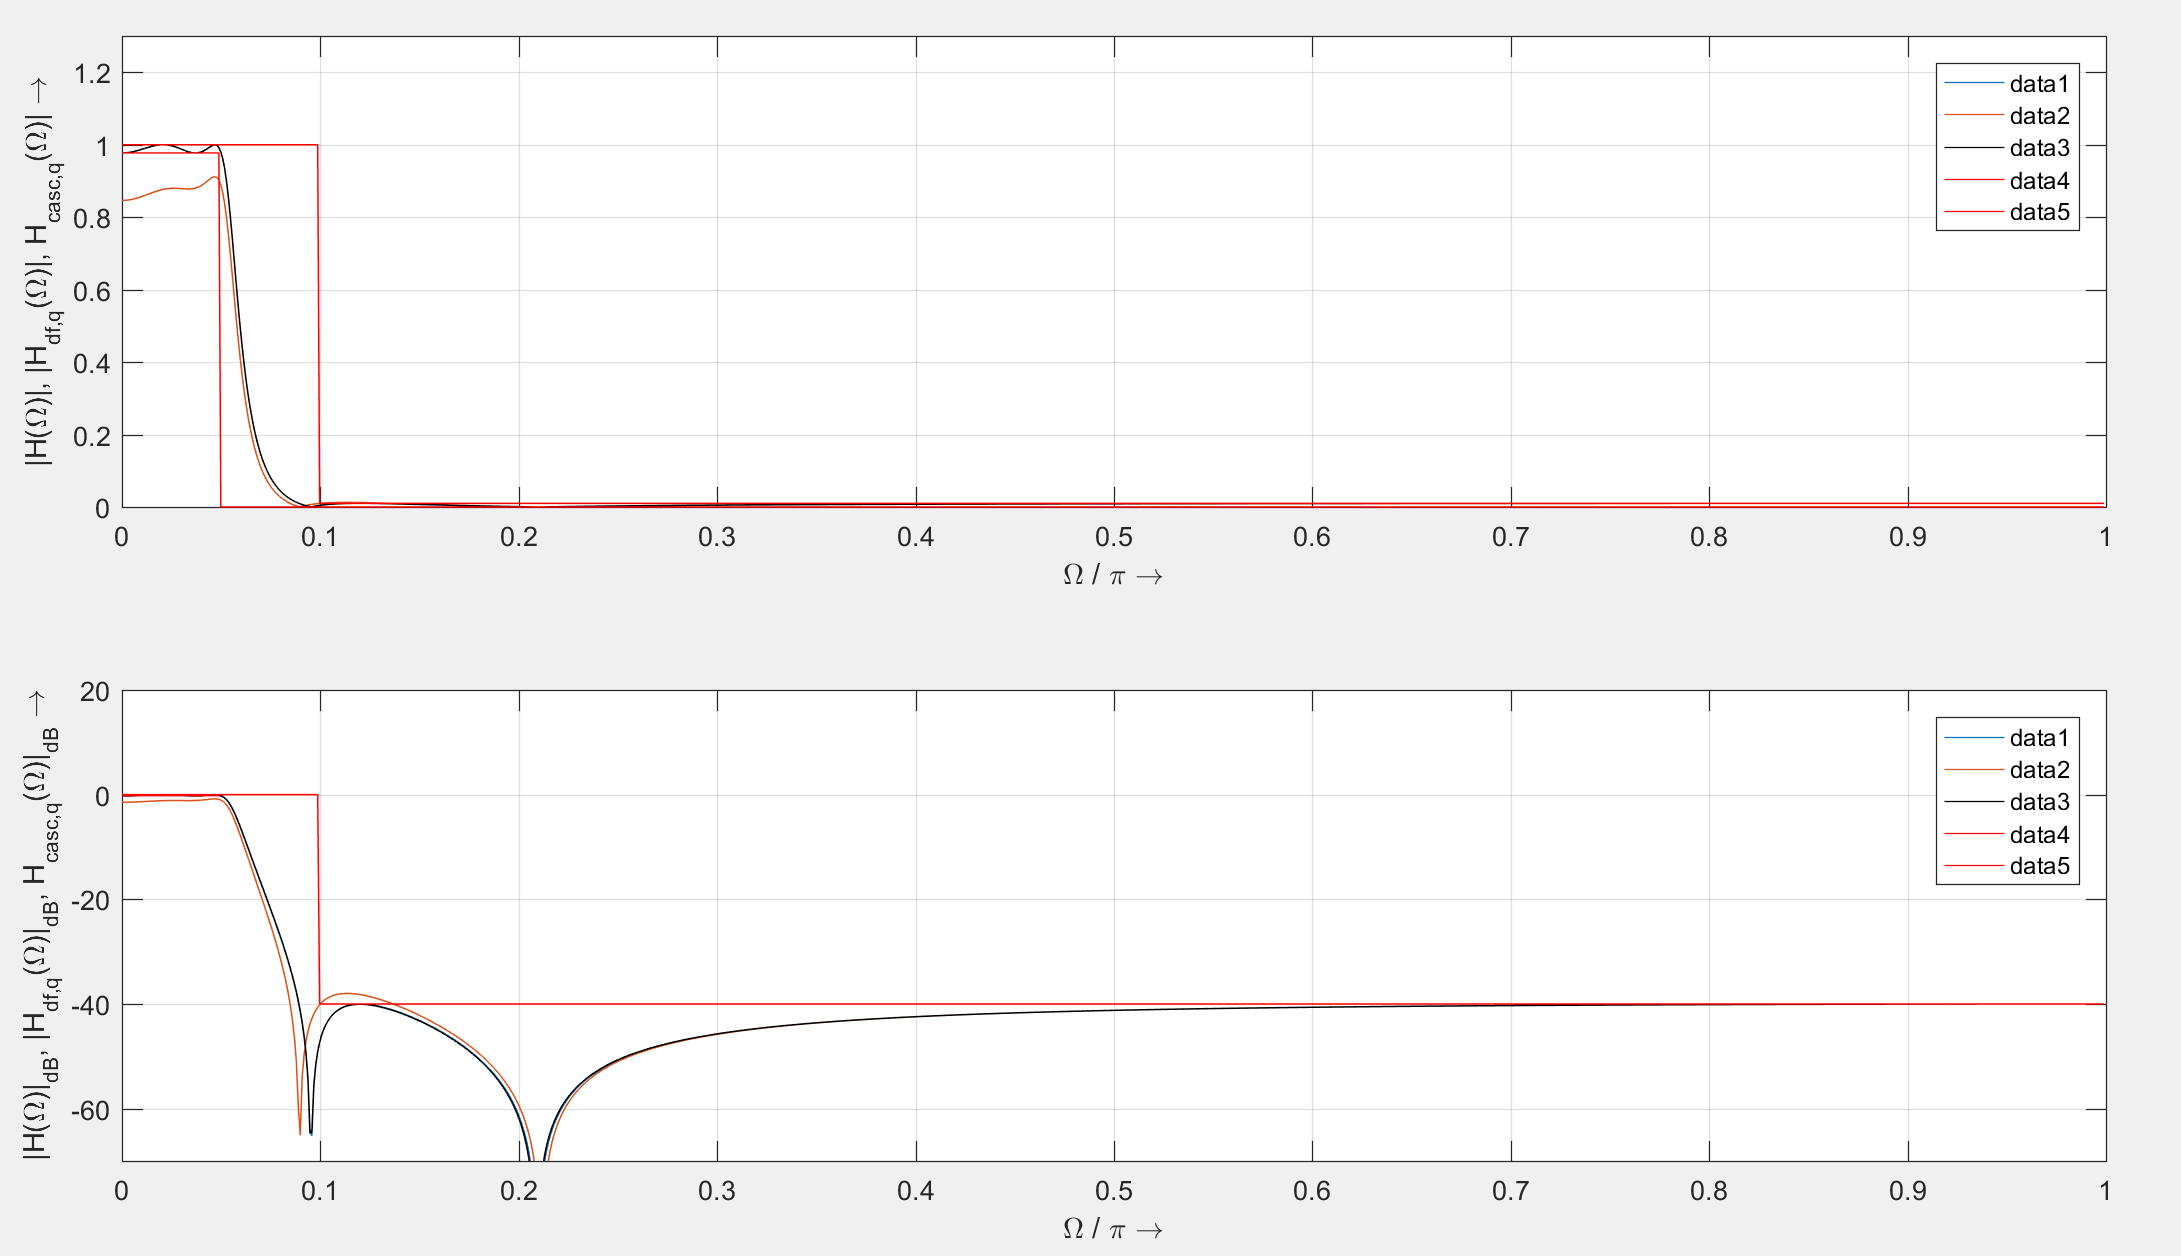
\includegraphics[scale=0.5]{UE02_3_16Bit.PNG}
\end{center}

\newpage

\subsection{Konsolenausgabe}

\sourceCode{UE02_3_output.txt}

\newpage

\subsection{Matlab-Skript}

\sourceCode{../../workspace/scd2_3.m}

\end{document}